\section{\mbox{Sequentielle}~\mbox{Bifurkation}~\mbox{visueller}~\mbox{Reizrepr"asentationen}}
\label{main}
\thispagestyle{plain}

Die in Abschnitt~\ref{unterschiede} vorgestellten Speziesunterschiede der
funktionalen Architektur des prim"aren visuellen Cortex laufen auf dem
ersten Blick dem Versuch einer einheitlichen Beschreibung ihrer Entstehung
zuwider.  Es ist jedoch eine plausible Annahme, da"s die Entstehung solcher
Reizrepr"asentationen in den untersuchten S"augetierarten vielleicht nicht
identischen, zumindest aber verwandten Regeln folgt
(vgl. Abschn.~\ref{plastizitaet}).  Im folgenden wird aus den in
Kapitel~\ref{modell} gewonnenen Einsichten "uber das elastische Netz ein
allgemeines Szenarium f"ur die Selbstorganisation visueller
Reizrepr"asentationen entwickelt, mit dessen Hilfe sich die in
Kapitel~\ref{biologie}, Abschnitt~\ref{unterschiede} beschriebenen
Ph"anomene einheitlich beschreiben lassen.

\subsection{Vorbetrachtungen}

Von verschiedenen Autoren wurden bereits m"ogliche Erkl"arungen dieser
Speziesunterschiede vorgeschlagen.  Es ist eine plausible Annahme, da"s die
Reichweite der lateralen Verbindungen zwischen den Neuronen einer
Zellschicht die Wellenl"ange eines kolumn"aren Musters determiniert. Diese
Vorstellung resultiert aus der "Uberlegung, da"s die Gr"o"se eines durch
einen Reiz hervorgerufenen Erregungsgebietes in einer Zellschicht mit
dieser Verbindungsreichweite verkn"upft sein sollte.  Modellsimulationen
mit unterschiedlichen lateralen Verbindungsreichweiten ergeben tats"achlich
Muster unterschiedlicher Wellenl"ange \cite{swindale:1992}.

Basierend auf dieser Annahme wurde zur Erkl"arung der verschiedenen
Wellenl"angen der OD-- und OP--Systeme vorgeschlagen, da"s sich jedes der
Systeme in einer eigenen neuronalen Schicht mit jeweils verschiedenen,
lateralen Verbindungsreichweiten zwischen den Neuronen ausbildet
\cite{loewel:1988}.  Die Autoren erwogen, da"s nicht nur die Wellenl"ange,
sondern auch die unterschiedlich ausgepr"agte ra"umliche Ordnung der Muster
(siehe Abb.~\ref{layout} und Abb.~\ref{odcorr}) mit der Gr"o"se der
lateralen Verbindungsreichweite korreliert sein k"onnte. In
Modellsimulationen der koordinierten Entwicklung von OD-- und OP--Karten
bedarf es jedoch zus"atzlicher Annahmen, um die beobachtete Anisotropie der
OD--Karte im Affen zu reproduzieren \cite{swindale:1992}.  Eine r"aumliche
Trennung der Muster verschiedener Wellenl"ange erschwert au"serdem die
Erkl"arung der lokalen geometrischen Beziehung zwischen den Mustern der
Okulardominanz und der Orientierungspr"aferenz, wie sie im visuellen Cortex
von Affen und Katzen beobachtet wird (vgl. Abschn.~\ref{90grad}).

In biologischen Systemen h"angt die Gr"o"se eines lokalen Erregungsgebietes
in einer bestimmten Zellschicht mindestens von zwei Faktoren ab: Der
Reichweite der lateralen Verbindungen der Neurone innerhalb einer
Zellschicht und der Ausdehnung der im prim"aren visuellen Cortex
terminierenden Axonen"aste.  Diese Axonen"aste stehen am Ende der
Nervenbahn (\emph{radiatio optica}, vgl. Abschn.~\ref{sehbahnkap}), die das
LGN mit dem Cortex verbindet.  Es gibt experimentelle Evidenz daf"ur, da"s
beide Gr"o"sen, sowohl die laterale Verbindungsreichweite als auch die
Ausdehnung der im Cortex terminierenden Axonen"aste, im Laufe der ersten
Lebenswochen abnehmen. Evidenz f"ur abnehmende laterale
Verbindungsreichweiten lieferten u.A. Untersuchungen am Frettchen
\cite{katz:1994}\footnote{Die Autoren dieser Arbeit diskutieren haupts"achlich
die Vergr"o"serung der langreichweitigen Verbindungen der Neurone. Jedoch
ist aus den Daten ersichtlich, da"s die lokale Verbindungsreichweite im
Laufe der Entwicklung abnimmt.}. Kleine und gro"se Axonen"aste in jungen und
adulten Katzen wurden von \citeasnoun{ferster:1978}
bzw. \citeasnoun{levay:1979} beobachtet.  Es ist also plausibel anzunehmen,
da"s die Ausdehnung eines typischen Erregungsgebietes im visuellen Cortex
im Laufe der Entwicklung abnimmt. Diese Annahme und das kritische Verhalten
des elastischen Netzes sind wichtige Vorraussetzungen f"ur das im folgenden
Abschnitt entwickelte Szenarium.
\setcounter{footnote}{1}

\subsection{Das sequentielle Bifurkationsszenarium}

\begin{figure}[t]
\begin{center}
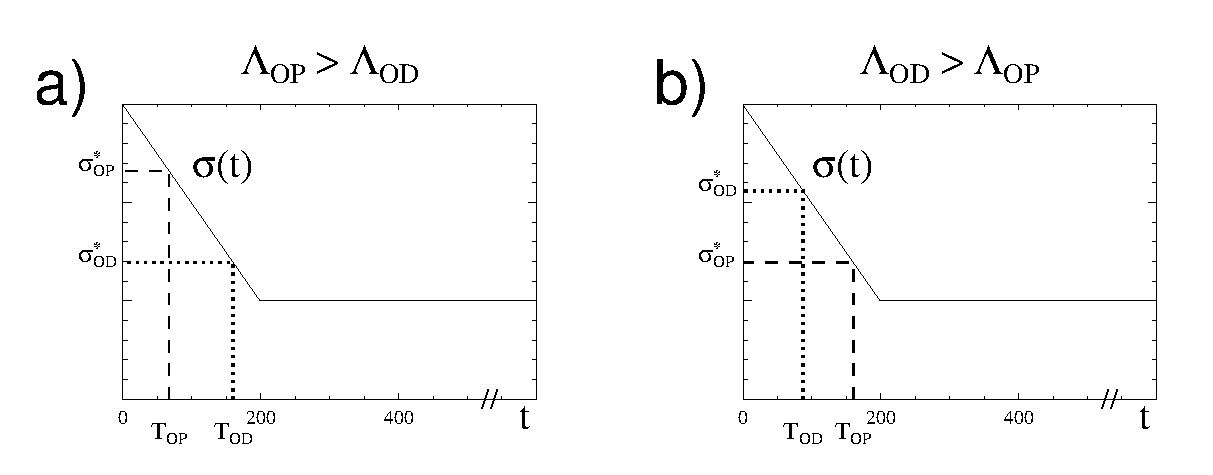
\epsfig{file=pics/seqbif.eps,width=\textwidth}
\caption{Skizze der in den Simulationen zur koordinierten Enstehung von
OD-- und OP--Mustern verwendeten Zeitentwicklung des
Modell--Parameters~$\sigma$ \textbf{a)} ``Katzen--"ahnliche'' Simulation:
Hier entsteht die Orientierungspr"aferenz zuerst, und hat daher die
gr"o"sere Wellenl"ange. \textbf{b)} ``Affen--"ahnliche'' Simulation: in
diesem Fall ensteht das Muster der Okulardominanz zuerst (und hat daher die
gr"o"sere Wellenl"ange).}
\label{zeitentwicklung}
\end{center}
\end{figure}

Wie in Kapitel~\ref{modell} dargestellt, existiert im elastischen Netz f"ur
jede emergierende kolumn"are Struktur eine unabh"angige, kritische
Kooperationsreichweite $\sigma_i^\ast$.  Diese wiederum wird durch die
Stimulusvarianz  in der entsprechenden Merkmalsraumdimension bestimmt. Die
kritischen Kooperationsreichweiten f"ur die Muster der
Orientierungspr"aferenz und die Okulardominanz werden also in der Regel
verschiedene Werte annehmen. Qualitativ sind dabei zwei F"alle zu
unterscheiden:

\begin{enumerate}
\item $\sigma_{\text{OD}}^\ast > \sigma_{\text{OP}}^\ast$ 
\item $\sigma_{\text{OD}}^\ast < \sigma_{\text{OP}}^\ast$ 
\end{enumerate}

Vor diesem Hintergrund hat die Annahme einer zeitabh"angigen, w"ahrend der
Entwicklung kontinuierlich schrumpfenden Kooperationsreichweite $\sigma(t)$
folgende Konsequenzen f"ur die Simulation der Dynamik~\eqref{endyn}: Ein
kontinuierlich abnehmendes $\sigma(t)$ unterschreitet die verschiedenen,
kritischen Kooperationsreichweiten $\sigma_i^\ast$ der 
kolumn"aren Muster \emph{sequentiell}. Zu jedem Zeitpunkt $t$, an dem
$\sigma(t)$ eine dieser kritischen Reichweiten $\sigma_i^\ast$
unterschreitet, wird die homogene L"osung in der entsprechenden Dimension
instabil; es bilden sich kolumn"are Muster mit einer durch das jeweilige
$\sigma_i^\ast$ determinierten Wellenl"ange.  Die unterschiedlichen
L"angenskalen verschiedener kolumn"arer Systeme werden also in eine
\emph{zeitliche Abfolge von Instabilit"aten} "ubersetzt. Dies bezeichnen
wir als \emph{sequentielles Bifurkationsszenarium}.  Den beiden oben
angef"uhrten Verh"altnissen von $\sigma_{\text{OD}}^{\phantom{\ast}}$ zu
$\sigma_{\text{OP}}^{\phantom{\ast}}$ entspricht damit (1.)
$\Lambda_{\text{OD}} > \Lambda_{\text{OP}}$ und (2.) $\Lambda_{\text{OD}} <
\Lambda_{\text{OP}}$.

Die in Affen und Katzen beobachteten, unterschiedlichen
Wellenl"angenverh"altnisse lassen sich mit dem sequentiellen
Bifurkationsszenarium also auf elegante Weise einheitlich erkl"aren: Das
sequentielle Bifurkationsszenarium sagt voraus, da"s sich in jeder Spezies
das Muster mit der gr"o"seren Wellenl"ange zuerst ausbildet
(vgl. Abb.~\ref{zeitentwicklung}). In Modellsimulation zum Szenarium
werden die genauen Wellenl"angenverh"altnisse notwendigerweise
reproduziert.  Inwieweit die Annahme einer unterschiedlichen
Entstehungsreihenfolge der OD-- und OP--Karten auch die r"aumliche Ordnung
dieser Karten erkl"aren kann, wird in den folgenden Abschnitten untersucht.

\subsection{Dynamische Umordnung der Okulardominanz}
\label{odord}

\begin{figure}[t]
\begin{center}
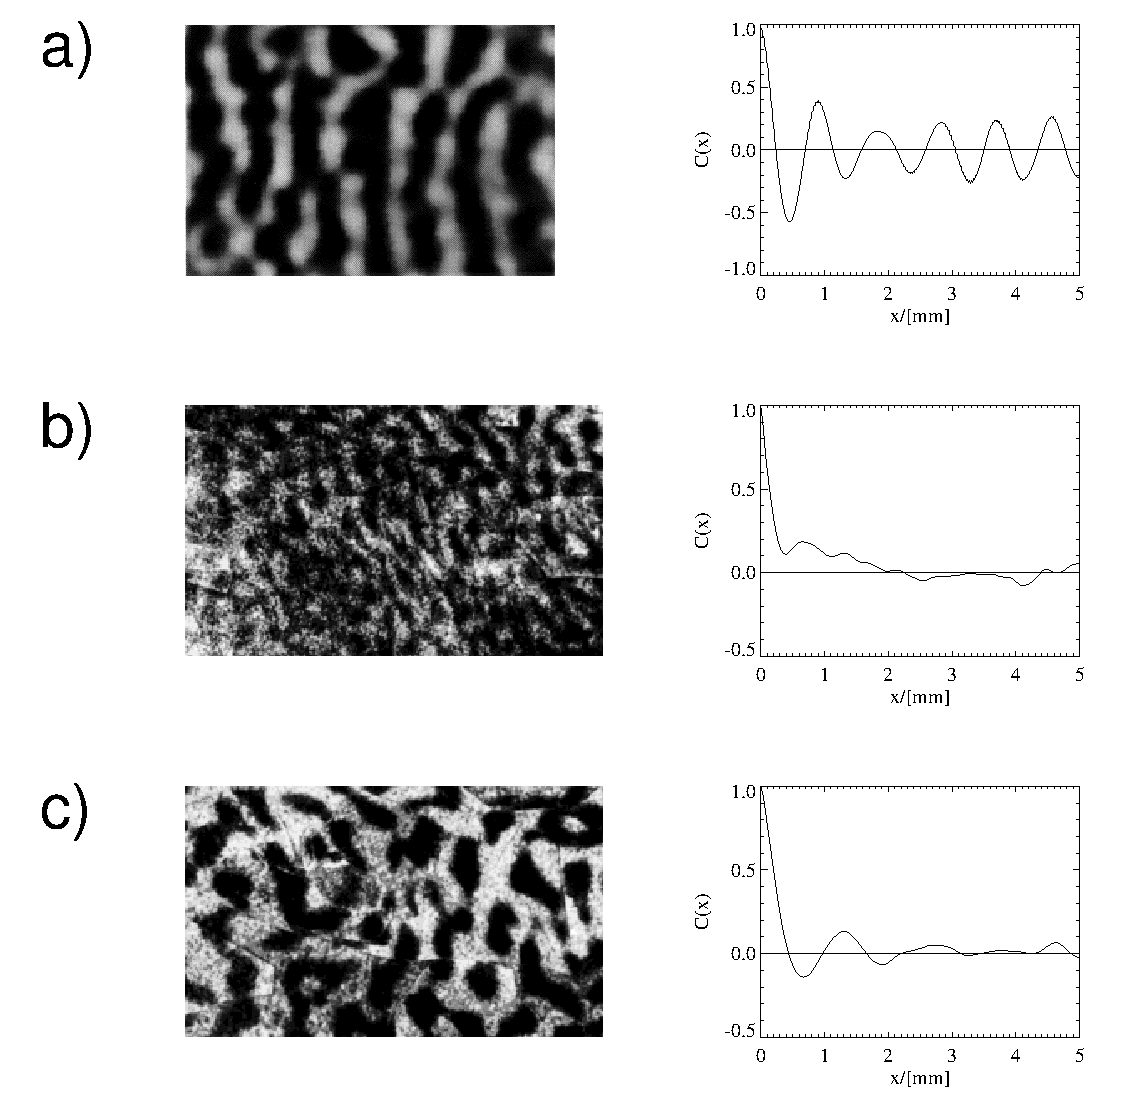
\epsfig{file=pics/od_corr.eps,width=11.9cm}
\end{center}
\caption{Die Bilder zeigen typische Auschnitte des OD--Musters aus V1 eines
Affen \protect\citeaffixed{grinvald:1991}{6.4mm$\times$4.3mm, optisches
Ableiten,} und aus A17 einer normalsichtigen und strabismischen Katze
\protect\citeaffixed{loewel:1987}{jeweils 5mm$\times$3mm, [$^3$H]--Prolin
Markierung,}. Neben jedem Bild ist die dazugeh"orige Autokorrelation
$C(\mathbf{r})\vert_{\mathbf{r}={x\choose 0}}$ gezeigt.}
\label{odcorr}
\end{figure}

\begin{figure}[t]
\begin{center}
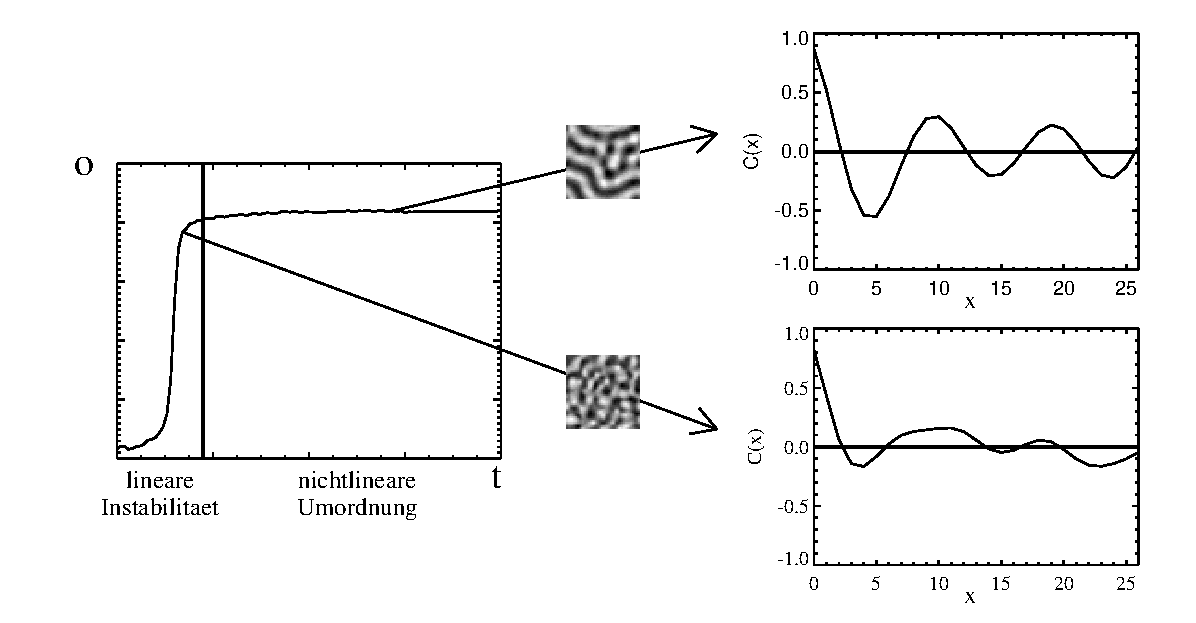
\epsfig{file=pics/umordnung.eps,width=\textwidth}
\end{center}
\caption{Simulation der Okulardominanz mit dem elastischen Netz. Links:
typische Entwicklung der Amplitude der instabilen L"osung. Rechts:
Autokorrelation eines typischen OD--Musters kurz und lange nach der
Instabilit"at.}
\label{umordnung}
\end{figure}

Das Muster der Okulardominanz im Affen zeigt einen hohen Grad r"aumlicher
Koh"arenz (vgl. Abschn.~\ref{unterschiede}): Die OD--Dom"anen bilden ein
System paralleler Streifen, die selten verzweigen und haupts"achlich
senkrecht zum Arealrand verlaufen \citeaffixed{levayetal:1985}{siehe
z.B.}. Um diese Ordnung des Musters zu quantifizieren wurde die
Autokorrelation

\begin{small}
\begin{equation}
C(\mathbf{r})=\left<\left(O(\mathbf{x+r})-\bar{O}\right)\ast\left(O(\mathbf{x})-\bar{O}\right)\right>_{\mathbf{x}\,\in\,\text{Bild}},\;\;\bar{O}=\left<O(\mathbf{x})\right>_{\mathbf{x}\,\in\,\text{Bild}}
\label{autocorr} 
\end{equation}
\end{small}

\noindent digitalisierter OD--Karten von Affen, strabismischen und
normalsichtigen Katzten berechnet.  Im gezeigten Ausschnitt aus der
OD--Karte des Affen sieht man die globale Vorzugsrichtung der Dom"anen
eutlich.  Dieser Augenschein wird durch die einige Perioden anhaltende
Modulation der Autokorrelation best"atigt (siehe Abb.~\ref{odcorr}).
Dagegen zerf"allt die Autokorrelation sowohl der OD--Karte der
strabismischen als auch der normalsichtigen Katze in allen Richtungen
schnell. Die Dom"anen dieser beiden Muster zeigen keine detektierbare
Vorzugsrichtung\footnote{Interessanterweise ist die Monokularit"at der
Zellen in A17 strabismischer Katzen st"arker ausgepr"agt als in V1 des
Affen (vgl. Abschn.~\ref{unterschiede}, Abb.~\ref{okuhist}).  Also l"a"st
sich weder der Grad der Monokularit"at der Neurone noch die Reichweite
ihrer lateralen Verbindungen zur Erkl"arung der unterschiedlichen
Anisotropie der OD--Muster in Katzen und Affen heranziehen.}.
\setcounter{footnote}{1}

Die in Simulationen aufgrund der Isotropie der Dynamik
hervorgebrachten Strukturen sind notwendigerweise statistisch isotrop
(siehe Abschn.~\ref{stabilitaet}).  Der ersten Etablierung eines solchen
Musters durch einen linearen Instabilit"atsmechanismus kann jedoch 
eine Phase der kontinuierlichen, nichtlinearen Umordnung folgen.  Simulationen der Entstehung von Okulardominanzkarten mit
dem elastischen Netz~\eqref{endyn} zeigen, da"s das Muster tats"achlich in
dieser nichtlinearen Umordnungsphase anisotrop wird und sich in ein System
paralleler Streifen umordnet (siehe Skizze in
Abb.~\ref{umordnung}).

\subsection{Ergebnisse numerischer Simulationen zum Szenarium}
\label{numerg}

Zur Erzeugung kolumn"arer Strukturen die sich durch das sequentielle
Bifurkationsszenarium ergeben wurde die Dynamik~\eqref{endyn} ausgehend vom
Anfangszustand $\mathbf{R}_0(\mathbf{x}) = (x,\, y,\, 0,\, 0,\, 0) $ f"ur
ein endliches Cortexareal $\cal T$ mit periodischen Randbedingungen
numerisch integriert (f"ur Details dazu siehe Anhang~\ref{anhang2}).

In einer Reihe von  Simulation  wurden die Stimulusvarianzen in den
Merkmalsdimensionen der Orientierungspr"aferenz und Okulardominanz  so
eingestellt, da"s nicht nur $\sigma^\ast_{\text{OP}}>\sigma^\ast_{\text{OD}}$
(und damit $\Lambda_{\text{OP}} > \Lambda_{\text{OD}}$,
vgl. Abb.~\ref{zeitentwicklung}a), sondern auch
das aus A17 der Katze bekannte Verh"altnis der Wellenl"angen beider
Muster (vgl.~Abschn.~\ref{unterschiede}, Abb.~\ref{wavelength})
erhalten wurde.  In Simulationen mit kontinuierlich schrumpfenden
$\sigma(t)$ entsteht dann das Muster der Orientierungspr"aferenz vor dem
Muster der Okulardominanz (siehe Abb.~\ref{opod}).

\begin{figure}[p]
\begin{center}
\begin{sideways}
\epsfig{file=pics/opod_rot.eps,height=\textwidth}
\end{sideways}
\end{center}
\caption{Momentaufnahmen der koordinierten Entwicklung von Okular\-do\-minanz--
und Orientierungskarten f"ur
$\sigma^\ast_{\text{OP}}>\sigma^\ast_{\text{OD}}$ (Szenarium
Abb.~\ref{zeitentwicklung}a). Die Farb--/Grauwertintensit"at spiegelt
die Amplitude der Strukturen wieder ($40\times 40$ Neurone mit periodischen
Randbedingungen, $\eta_{\text{rel}}=0.0025$,
$\sigma^\ast_{\text{OD}}=0.0837$, $\sigma^\ast_{\text{OP}}=0.1189$
$\Longrightarrow$ $\Lambda_{\text{OD}}/\Lambda_{\text{OP}}=4/5$).}
\label{opod}
\end{figure}

\begin{figure}[p]
\begin{center}
\begin{sideways}
\epsfig{file=pics/odop_rot.eps,height=\textwidth}
\end{sideways}
\end{center}
\caption{Momentaufnahmen wie oben, jedoch in einer Simulation mit
$\sigma^\ast_{\text{OD}}>\sigma^\ast_{\text{OP}}$, ensprechend des Szenariums in
Abb.~\ref{zeitentwicklung}b ($40\times 40$ Neurone mit
periodischen Randbedingungen, $\eta_{\text{rel}}= 0.0025$,
$\sigma^\ast_{\text{OD}}=0.0976$, $\sigma^\ast_{\text{OP}}=0.0679$
$\Longrightarrow$ $\Lambda_{\text{OD}}/\Lambda_{\text{OP}}=6/5$).}
\label{odop}
\end{figure}

In einer weiteren Reihe von Simulationen wurde die zweite Variante des
Szenariums (Abb.~\ref{zeitentwicklung}b) untersucht: Die Varianzen der
Reizverteilungen in den Merkmalsdimensionen wurden entsprechend des f"ur
den Affen geltenden Wellen\-l"angen\-ver\-h"altnisses gew"ahlt. Da hier
$\Lambda_{\text{OD}} > \Lambda_{\text{OP}}$ ist, entsteht in Simulationen
mit kontinuierlich schrumpfenden~$\sigma(t)$ also das Muster der
Okulardominanz vor dem Muster der Orientierungspr"aferenz (siehe
Abb.~\ref{odop}).

Abbildung~\ref{simres} stellt die Endkonfigurationen der in den
Abbildungen~\ref{opod} und \ref{odop} gezeigten, typischen
Simulationsergebnisse zu diesem Szenarium nocheinmal vergleichend vor.  Im
einen Fall (Abb.~\ref{opod} und Abb.~\ref{simres}, links) bildet die
Okulardominanz perlige Dom"anen. Die Grenzlinien dieser Dom"anen verlaufen
dabei oft geschlossen um die Singularit"aten der Orientierungskarte.  Im
anderen Fall bildet das Muster der Okulardominanz ein System ausgedehnter
Streifen, die selten verzweigen und "uber weite Abschnitte parallel
verlaufen (Abb.~\ref{odop} und Abb.~\ref{simres}, rechts).
In beiden F"allen des Szenariums stimmen die Ergebnisse aller durchgef"uhrten
Simulationen gut mit den experimentell beobachteten Karten "uberein. Das
nicht nur die Wellenl"angenverh"altnisse sondern, wie in Abb.~\ref{simres}
gezeigt, auch die unterschiedlichen Layouts der Muster korrekt reproduziert
werden, bedarf einer zus"atzlichen Erkl"arung.

\begin{figure}[t]
\begin{center}
\begin{minipage}[t]{6.2cm}
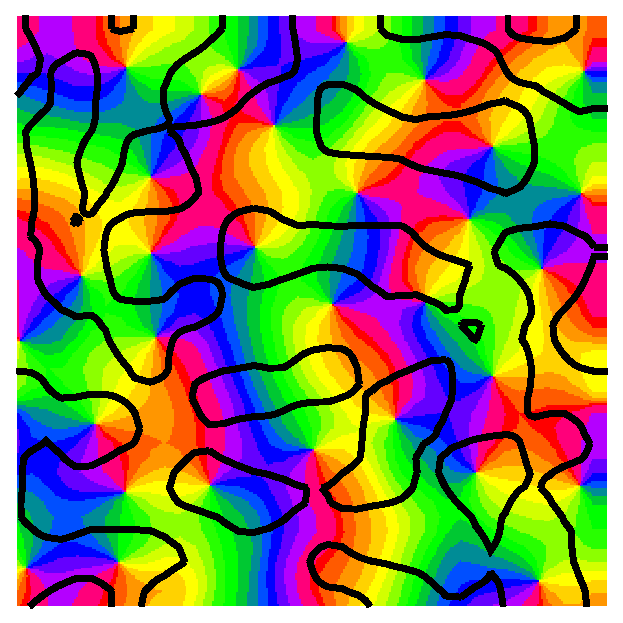
\epsfig{file=pics/op+od.eps,width=6.2cm} 
\end{minipage}
\hskip0.4cm 
\begin{minipage}[t]{6.2cm}
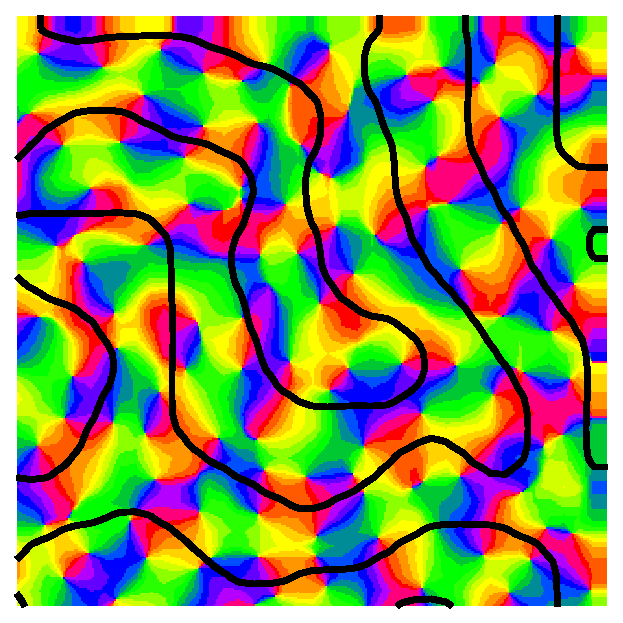
\epsfig{file=pics/od+op.eps,width=6.2cm} 
\end{minipage}
\end{center}
\caption{Vorhersage des funktionalen Layouts von Okulardominanz-- und 
Orientierungspr"aferenz--Karten f"ur die Katze (links, Ergebnis der in
Abb.~\ref{opod} gezeigten Simulation) und den Affen (rechts, Ergebnis der
in Abb.~\ref{odop} gezeigten Simulation).  Die Abbildungen zeigen eine
"Uberlagerung der Iso--Orientierungsdom"anen (farbig) mit den Grenzenlinien
der Okulardominanzkolumnen (schwarz).}
\label{simres}
\end{figure}

\begin{figure}[p]
\begin{center}
\begin{sideways}
\epsfig{file=pics/oddev.eps,height=12cm}
\end{sideways}
\end{center}
\caption{Momentaufnahmen der Weiterentwicklung einer Okulardominanzkarte.
Die am Anfang gezeigte Karte entstand in einer typischen Simulation mit
$\sigma^\ast_{\text{OP}}>\sigma^\ast_{\text{OD}}$. Ihre Weiterentwicklung in
dieser Simulation zeigt die untere Reihe. Die obere Reihe zeigt die
Weiterentwicklung der Karte \emph{ohne} das Muster der
Orientierungspr"aferenz (beide Reihen: $40\times 40$ Neurone,
$\sigma(t)=\sigma^\ast_{\text{OD}}*0.9$, $\eta_{\text{rel}}=0.001$).}
\label{oddev}
\end{figure}

\begin{figure}[p]
\begin{center}
\begin{sideways}
\epsfig{file=pics/angledev.eps,width=9cm}
\end{sideways}
\end{center}
\caption{Typische Entwicklung der geometrischen Beziehung zwischen den
Iso--Orientierungslinien und den Okulardominanz--Grenzlinien im Anschlu"s
an die prim"are Etablierung beider Strukturen.}
\label{angledev}
\end{figure}

Die Wechselwirkung der verschiedenen kolumn"aren Strukturen im elastischen
Netz f"uhrt zu einer Reproduktion der in Abschnitt~\ref{90grad}
vorgestellten, geometrischen Beziehung zwischen den
Iso--Orientierungslinien und den Grenzlinien der Okulardominanz
(vgl. \citeasnoun{erwin:1995} und Abb.~\ref{odop_hist}, links). Daher
erschient die Annahme plausibel, da"s auch im visuellen Cortex von Katzen
und Affen diese geometrische Beziehung Ergebnis einer dynamischen
Interaktion der OD-- und OP--Karten ist. In diesem Fall w"are das Muster
der Okulardominanz in der Katze ``versklavt'': Die fr"uher entstandene
Orientierungskarte w"urde die Umorganisation der Okulardominanz in ein
System parallerel B"ander mit Vorzugsrichtung verhindern.  Durch die
Wechselwirkung beider Muster im Modell bildet sich in diesem Fall die
sp"ater entstehende Okulardominanzkarte so aus, da"s ihre Grenzlinien
h"aufig geschlossene Kurven um Pinwheels bilden. Dies erf"ullt die
Randbedingung der in Abschnitt~\ref{90grad} vorgestellten, geometrischen
Beziehung beider Strukturen. 

Um diese Hypothese der Versklavung der Okulardominanz zu testen, wurde nach
der Entstehung beider Muster in Simulationen mit
$\sigma^\ast_{\text{OP}}>\sigma^\ast_{\text{OD}}$ untersucht, wie sich die
Okulardominanzkarte \emph{mit} bzw. in Abwesenheit der Orientierungskarte
weiterentwickelt. Wie Abbildung~\ref{oddev} an einem Beispiel zeigt, ordnet
sich der identische Ausgangszustand der Okulardominanzkarte ohne
Orientierungskarte in ein System paralleler B"ander mit Vorzugsrichtung um.
Unter Br"ucksichtigung der Randbedingung stumpfer Schnittwinkel zwischen
Iso--Orientierungslinien und Okulardominanz--Grenzlinien l"a"st sich also
in der Katze das Layout der Muster durch ihre sequentielle Enstehung
erkl"aren.  Ein wie im Affen beobachtetes, r"aumlich koh"arentes Muster der
Okulardominanz dagegen kann ebenfalls nur durch dynamische Umordnung in
Abwesenheit des Musters der Orientierungspr"aferenz entstehen
(vgl. Abschn.~\ref{odord}).  Aus unseren Simulationen folgt also, da"s die
Wechselwirkung der Strukturen ihr Erscheinungsbild entscheidend
beeinflu"st.

Berechnet man, wie in Abschnitt~\ref{90grad} dargelegt, die Verteilung der
Schnittwinkel zwischen den Iso--Orientierungslinien und den Grenzlinien der
Okulardominanz f"ur mehrere Konfigurationen im Zuge der Entwicklung, so
zeigt sich, das diese geometrische Beziehung beider Muster im Modell erst
in einem Zeitraum nach der prim"aren Etablierung der Muster realisiert
wird (ein Beispiel daf"ur zeigt Abb.~\ref{angledev}).  Dies wird in allen
durchgef"uhrten Simulationen der koordinierten Entwicklung von OD-- und
OP--Karten ungeachtet ihrer Entstehungsreihenfolge beobachtet und zeigt,
da"s diese geometrische Beziehung beider Muster Resultat eines dynamischen
Umordnungsprozess in der nichtlinearen Phase der Entwicklung ist.
